\documentclass[12pt]{article}
\usepackage{graphicx}
\usepackage{enumitem}
\usepackage[margin=0.75in]{geometry}
\usepackage{float}
\usepackage{listings}
\usepackage{xcolor}

\lstset{
  language=SQL,
  basicstyle=\ttfamily,
  keywordstyle=\bfseries\color{blue},
  commentstyle=\color{gray},
  stringstyle=\color{green!50!black},
  showstringspaces=false,
  numbers=left,
  numberstyle=\tiny,
  frame=single,
  backgroundcolor=\color{gray!10},
  breaklines=true,
}


\begin{document}

\title{ 
	DBMS-1\\
	Assignment 1:\\
    Report
}
\author{\textbf{Waghmare Aditya Abhaykumar}\\
    CS22BTECH11061}
\date{November 20, 2023}
\maketitle


\begin{enumerate}[label=\textbf{\arabic*:}, left=0pt, labelsep=10pt, align=left, parsep=0pt, itemsep=10pt]
    %1
    \item Find the top-3 instructors who have have taught most number of distinct courses from

        \begin{enumerate}[label=\textbf{\alph*.}, align=left, parsep=0pt, itemsep=10pt]
            %a
            \item Across all departments
            \\ \textbf{Query:}
            \begin{lstlisting}
SELECT instructor.id AS instructor_id, instructor.name AS instructor_name
FROM instructor
INNER JOIN teaches ON teaches.id = instructor.id
GROUP BY instructor.id
ORDER BY COUNT(DISTINCT teaches.course_id) DESC
LIMIT 3;
            \end{lstlisting}

            \\ \textbf{Output:}
            \begin{figure}[H]
                % \centering
                \hspace{60pt}
                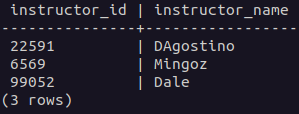
\includegraphics[width=0.4\textwidth]{images/1_a.png}
                \caption{Output for 1.a}
            \end{figure}

            %b
            \item Statistics department  
            \\ \textbf{Query:}
            \begin{lstlisting}
SELECT instructor.id AS instructor_id, instructor.name AS instructor_name
FROM instructor
INNER JOIN teaches ON teaches.id = instructor.id 
WHERE instructor.dept_name = 'Statistics'
GROUP BY instructor.id
ORDER BY COUNT(DISTINCT teaches.course_id) DESC
LIMIT 3;
            \end{lstlisting}

            \\ \textbf{Output:}
            \begin{figure}[H]
                % \centering
                \hspace{60pt}
                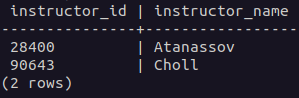
\includegraphics[width=0.4\textwidth]{images/1_b.png}
                \caption{Output for 1.b}
            \end{figure}
        \end{enumerate}
    
    \vspace{25pt}
    % 2
    \item Print teaching record of the instructor who has the highest salary, 
    showing the instructor department name, course identifier, course title, section number, semester, year and total enrollment. 
    Sort your result by course\_id, year, semester in ascending order. 
    \\ \textbf{Query:}
    \begin{lstlisting}
SELECT instructor.dept_name, teaches.course_id, course.title, section.sec_id, teaches.semester, teaches.year, total_enrollments
FROM instructor 
LEFT JOIN teaches ON teaches.id = instructor.id
LEFT JOIN course ON course.course_id = teaches.course_id
LEFT JOIN
    (SELECT course_id AS c_id, COUNT(id) AS total_enrollments
    FROM takes 
    GROUP BY course_id)
ON c_id = course.course_id
LEFT JOIN section ON section.course_id = course.course_id
WHERE instructor.id = (SELECT id FROM instructor ORDER BY salary DESC LIMIT 1)
ORDER BY teaches.course_id, teaches.year, teaches.semester;
    \end{lstlisting}

    \\ \textbf{Output:}
    \begin{figure}[H]
        \centering
        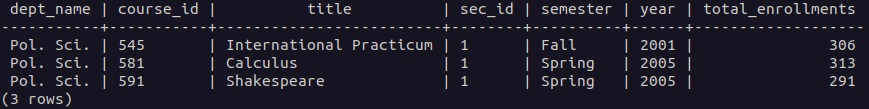
\includegraphics[width=1\textwidth]{images/2.png}
        \caption{Output for 2}
    \end{figure}

    \vspace{25pt}
    % 3
    \item Print history of the course with course\_id = 362. For each offering of the course, print course id, 
    course title, course department name, instructor name, number of registered students, section id, 
    semester, year and timetable slot. Sort your result by year in descending order.   
    \\ \textbf{Query:}
    \begin{lstlisting}
SELECT DISTINCT course.course_id, course.title, course.dept_name, instructor.name AS instructor_name, registered, teaches.sec_id, teaches.semester, teaches.year, section.time_slot_id
FROM course
LEFT JOIN teaches ON course.course_id = teaches.course_id
LEFT JOIN 
    (SELECT course_id, year, semester, COUNT(id) AS registered
    FROM takes
    GROUP BY course_id, year, semester) 
    AS take
ON (take.course_id = course.course_id and take.semester = teaches.semester and take.year = teaches.year)
LEFT JOIN instructor ON instructor.id = teaches.id
LEFT JOIN section ON (course.course_id = section.course_id and teaches.sec_id = section.sec_id and teaches.semester = section.semester and teaches.year = section.year) 
WHERE course.course_id = '362'
ORDER BY teaches.year DESC;
    \end{lstlisting}

    \\ \textbf{Output:}
    \begin{figure}[H]
        \centering
        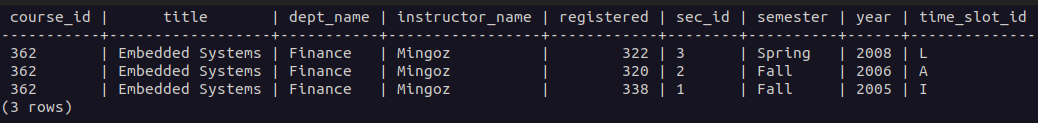
\includegraphics[width=1\textwidth]{images/3.png}
        \caption{Output for 3}
    \end{figure}

    \vspace{25pt}
    % 4
    \item  For the course\_id 319 that was offered in 2003, find the count of out of department student registration. 
    \\ \textbf{Query:}
    \begin{lstlisting}
SELECT COUNT(takes.id) AS out_of_department_student_registrations
FROM takes
LEFT JOIN student ON student.id = takes.id
LEFT JOIN course ON course.course_id = takes.course_id
WHERE course.course_id = '319' and year = 2003 and student.dept_name != course.dept_name;
    \end{lstlisting}

    \\ \textbf{Output:}
    \begin{figure}[H]
        % \centering
        \hspace{30pt}
        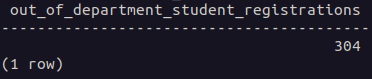
\includegraphics[width=0.4\textwidth]{images/4.png}
        \caption{Output for 4}
    \end{figure}

    \vspace{25pt}
    % 5
    \item Find top-3 students who have registered for the highest number of course credits. Order by total 
    credits and name. Print student id, name, department and total credits (Compute it from the takes 
    and course tables. Do not use tot\_credit in the student table.) 
    \\ \textbf{Query:}
    \begin{lstlisting}
SELECT student.id, name, student.dept_name, SUM(credits) AS total_credits
FROM student
LEFT JOIN takes ON takes.id = student.id
LEFT JOIN course ON course.course_id = takes.course_id
GROUP BY student.id
ORDER BY total_credits DESC, name 
LIMIT 3;
    \end{lstlisting}

    \\ \textbf{Output:}
    \begin{figure}[H]
        % \centering
        \hspace{30pt}
        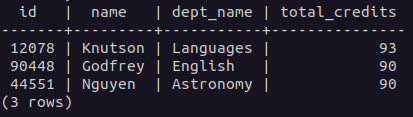
\includegraphics[width=0.6\textwidth]{images/5.png}
        \caption{Output for 5}
    \end{figure}

    \vspace{25pt}
    % 6
    \item Find the distinct set of courses that were not offered during 2003 and 2004. 
    Print the course id and title. Sort your result by course id in ascending order.    
    \\ \textbf{Query:}
    \begin{lstlisting}
SELECT DISTINCT course_id, title
FROM course
WHERE course_id NOT IN
    (SELECT DISTINCT course_id
    FROM teaches
    WHERE year = 2003 OR year = 2004)
ORDER BY course_id;
    \end{lstlisting}

    \\ \textbf{Output:}
    \begin{figure}[H]
        % \centering
        \hspace{30pt}
        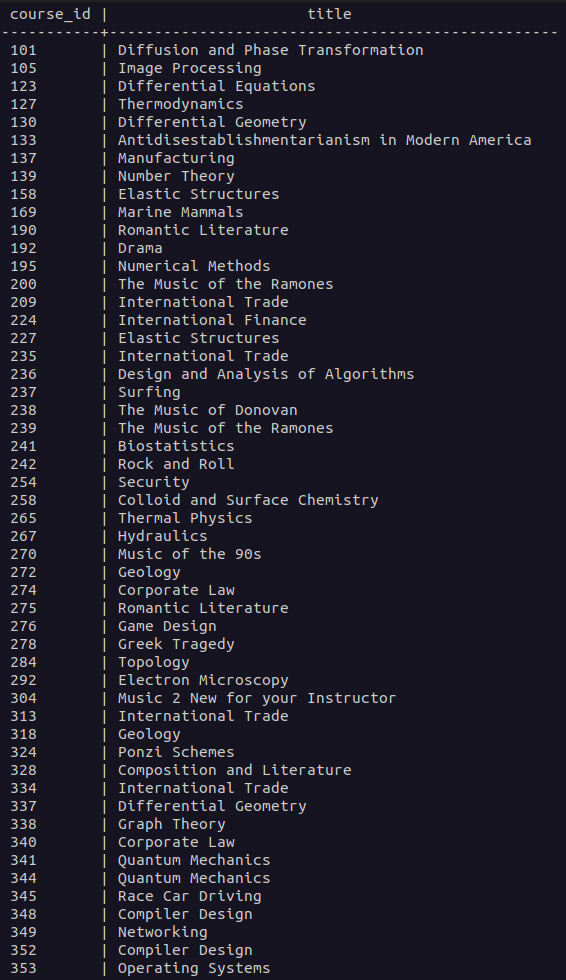
\includegraphics[width=0.7\textwidth]{images/6_1.png}
        \caption{Output for 6\_1}
    \end{figure}

    \begin{figure}[H]
        % \centering
        \hspace{30pt}
        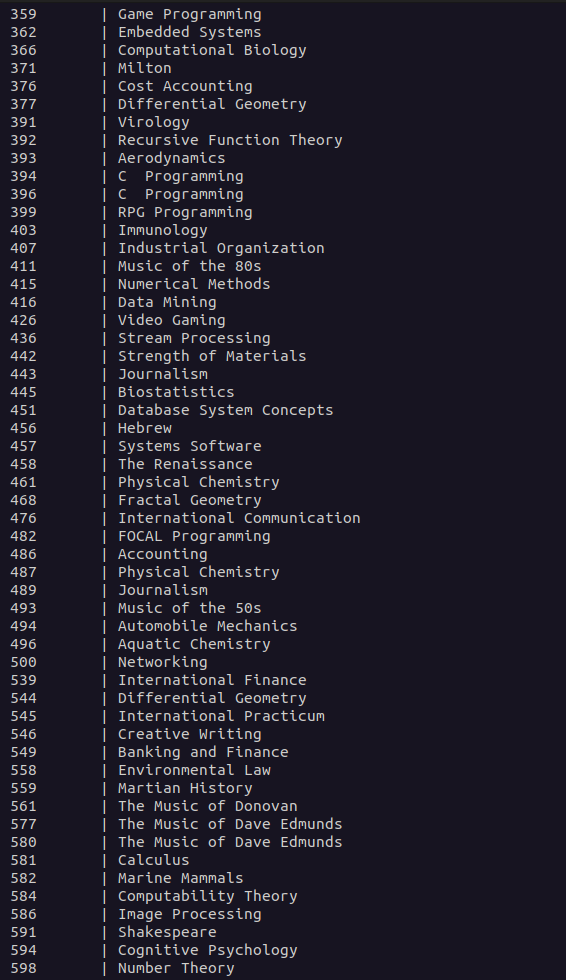
\includegraphics[width=0.7\textwidth]{images/6_2.png}
        \caption{Output for 6\_2}
    \end{figure}

    \begin{figure}[H]
        % \centering
        \hspace{30pt}
        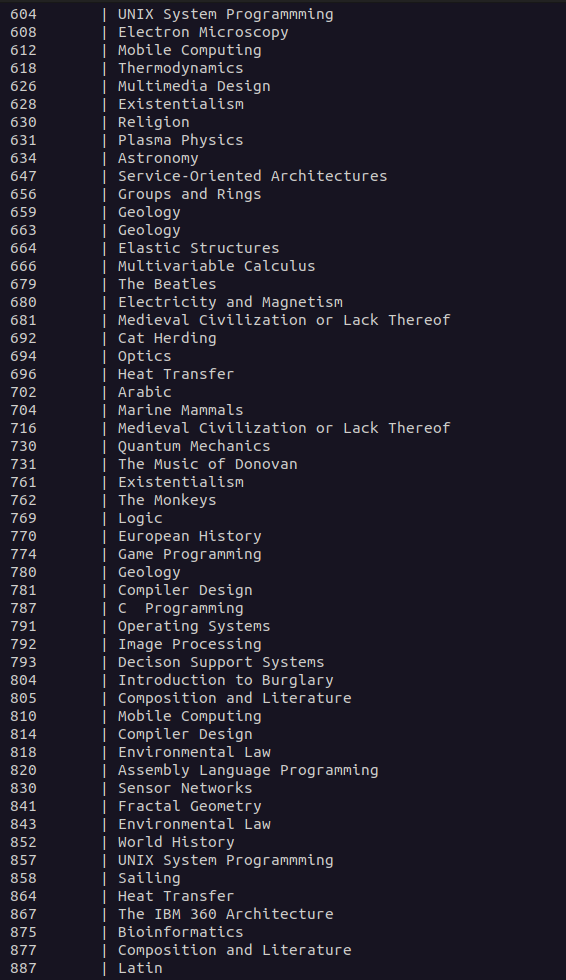
\includegraphics[width=0.7\textwidth]{images/6_3.png}
        \caption{Output for 6\_3}
    \end{figure}

    \begin{figure}[H]
        % \centering
        \hspace{30pt}
        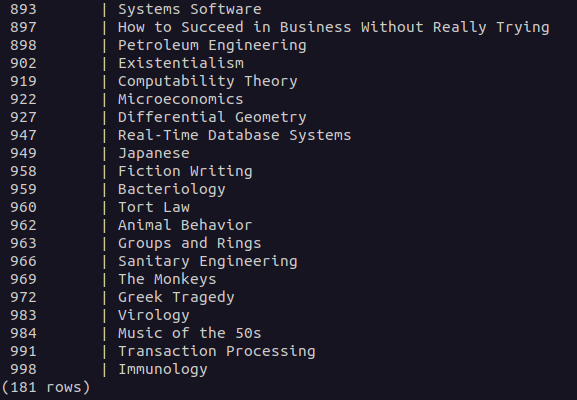
\includegraphics[width=0.7\textwidth]{images/6_4.png}
        \caption{Output for 6\_4}
    \end{figure}

    \vspace{25pt}
    % 7
    \item Find the courses that were offered for the first time most recently in terms of year. 
    Print the course id, title, instructor, year. Sort your result by course id in ascending order. 
    [Find the most recent year when a course was offered for the first time. 
    If there are more than one course offered that year for the first time, then print all of them.]
    \\ \textbf{Query:}
    \begin{lstlisting}
SELECT course.course_id AS course__id, course.title, instructor.name AS instructor_name, teaches.year
FROM course
INNER JOIN teaches ON teaches.course_id = course.course_id
LEFT JOIN instructor ON instructor.id = teaches.id
WHERE teaches.year IN
        (SELECT MAX(year)
        FROM teaches
        GROUP BY course_id
        HAVING COUNT(DISTINCT year) = 1
        ORDER BY MAX(year) DESC
        LIMIT 1)
    AND course.course_id IN
        (SELECT teaches.course_id
        FROM teaches
        GROUP BY course_id
        HAVING COUNT(DISTINCT teaches.year) = 1)
ORDER BY course.course_id;
    \end{lstlisting}

    \\ \textbf{Output:}
    \begin{figure}[H]
        % \centering
        \hspace{30pt}
        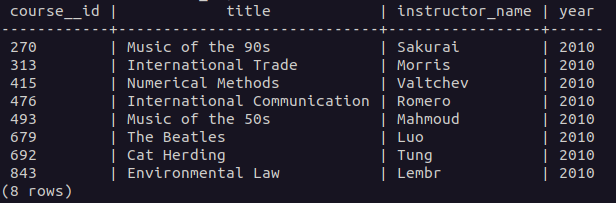
\includegraphics[width=0.6\textwidth]{images/7.png}
        \caption{Output for 7}
    \end{figure}

    \vspace{25pt}
    % 8
    \item Find all the courses whose title has more than 15 characters and have a 'sys' as substring in the title. 
    Consider case insensitive matching. 'sys', 'Sys', etc are all fine. 
    Print the course id and title. Sort result by course id.
    \\ \textbf{Query:}
    \begin{lstlisting}
SELECT course_id, title 
FROM course
WHERE LENGTH(title) > 15 AND title ILIKE '%sys%'
ORDER BY course_id;
    \end{lstlisting}

    \\ \textbf{Output:}
    \begin{figure}[H]
        % \centering
        \hspace{30pt}
        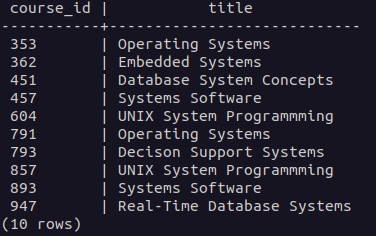
\includegraphics[width=0.4\textwidth]{images/8.png}
        \caption{Output for 8}
    \end{figure}

    \vspace{25pt}
    % 9
    \item Find the department that offers the highest average salary to instructors.
    \\ \textbf{Query:}
    \begin{lstlisting}
SELECT dept_name, avg(salary) AS avg_salary
FROM instructor
GROUP BY dept_name
ORDER BY avg_salary DESC
LIMIT 1;
    \end{lstlisting}

    \\ \textbf{Output:}
    \begin{figure}[H]
        % \centering
        \hspace{30pt}
        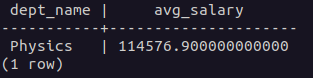
\includegraphics[width=0.4\textwidth]{images/9.png}
        \caption{Output for 9}
    \end{figure}

    \vspace{25pt}
    % 10
    \item Find all instructors who taught at most once in 2003. 
    (Didn't teach any course in 2003 or taught just one course in 2003). 
    Print instructor id, name and department. Sort your result by instructor id.
    \\ \textbf{Query:}
    \begin{lstlisting}
SELECT instructor.id, instructor.name, instructor.dept_name
FROM instructor
LEFT JOIN
    (SELECT teaches.id AS teaches_id, COUNT(course_id) AS taught
    FROM teaches
    WHERE year = 2003
    GROUP BY teaches.id)
ON teaches_id = instructor.id
WHERE taught = 1 OR taught IS NULL
ORDER BY instructor.id;
    \end{lstlisting}

    \\ \textbf{Output:}
    \begin{figure}[H]
        % \centering
        \hspace{30pt}
        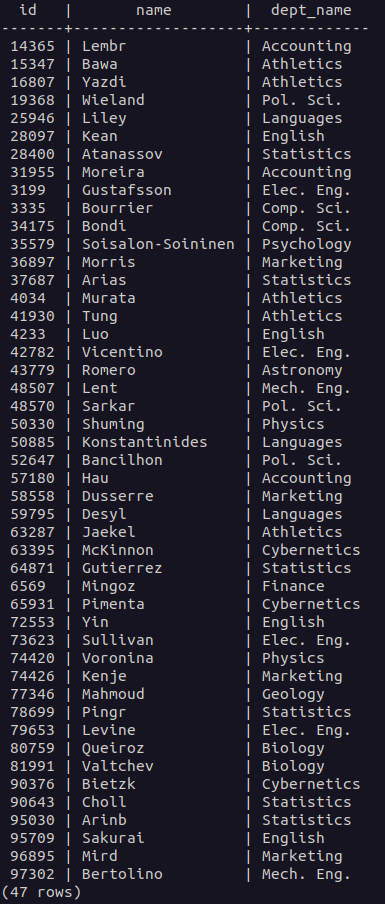
\includegraphics[width=0.5\textwidth]{images/10.png}
        \caption{Output for 10}
    \end{figure}


\end{enumerate}

\end{document}